\section{Methods}
\label{sec:Methods}
The goals of our methods are (i)~to make it possible to use CTC-based models for a reliable evaluation of GOP, (ii)~to reduce the sensitivity of GOP to precise speech segmentation and to consider the uncertainty of phonetic alignment, (iii)~to introduce context awareness into the definition of GOP and (iv)~to extend the method of GOP to allow for detecting insertion and deletion errors as well as substitutions.

To achieve these goals we propose two methods that will be detailed in Section~\ref{sec:gop-self-segmentation} and \ref{sec:gop-segmentation-free}.
%In this section we introduce the methods and motivate them theoretically.
%In Section~\ref{sec:experiments} and \ref{sec:results} we prove their effectiveness with empirical results.

\subsection{Self-alignment GOP (GOP-SA)}
%\subsection{Self-segmentation based GOPGOP-CTC-Align: The Forced-aligned CTC-Based GOP}
\label{sec:gop-self-segmentation}
Firstly, we consider the problem of mismatch between the segmentation of speech into phonetic units and the activations of the models used for GOP estimation as mentioned in Section~\ref{sec:alignment_issues}.
This phenomenon is exemplified in Figure~\ref{fig:illustration-alignment-problems} and is especially critical for CTC trained models (right plots) which exhibit peaky activations for each phoneme that may not correspond in time with the corresponding speech segment.
In order to address the problem, we propose to use the same GOP definition as for DNN models (Eq.~\ref{eqa:gop-dnn}) but to perform the alignment of the target segment ($t_1,t_2$) based on the same model used for GOP evaluation instead of an external forced aligner.
We refer to this method as self-alignment GOP (GOP-SA).
%that takes advantage of the peaky outputs of the model to produce an alignment that is consistent with the phonemes under assessment.
Figure~\ref{fig:illustration-alignment-problems} shows this alignment with red dashed vertical lines for the CTC-Loss trained models.
We want to stress that the goal of alignment in this method is not to find the segment corresponding to the target phone, but, rather, to find the activations of the model corresponding to the target phone.


%The GOP-CTC-Align shares the same definition of GOP-DNN-Avg (Eq.~\ref{eqa:gop-dnn}), that we repeat here for convenience:
%\begin{equation}
%    \label{eqa:gop-ctc-align}
%   \text{GOP-CTC-Align}(l_i)= \sum_{t=t_1}^{t_2}\log\left({\mathit{p}(l_i|O_t)} \right) / {|t_2 - t_1|}
%\end{equation}
%However, whereas the segmentation ($t_1, t_2$) in GOP-DNN-Avg was obtained with an external forced aligner, in GOP-CTC-Align we propose to use the same activations from the model to estimate $t_1$ and $t_2$.
%The rationale is that models trained with CTC exhibit peaky activations for each phoneme that may not correspond in time with the corresponding speech segment (see Figure~\ref{fig:illustration-alignment-problems}, right for examples).
We hypothesize that using CTC-based models for GOP would reduce the impact of the alignment errors due to mispronunciations which we mentioned in Sec.\ref{sec:alignment_issues}.
We will show that this method leads to improvements in MDD accuracy not only for the peaky models it was designed for, but for all the other models we have tested.


%It is the same as the definition of GOP-DNN-Avg in Eq.\eqref{eqa:gop-dnn} but differs in that the segmentation $t_1$ and $t_2$ is obtained from running forced alignment with the trained CTC-based model instead of an external context-independent aligner, even though, as discussed earlier, the external aligner could generate more accurate alignment with respect to acoustic evidence. 
%Unlike training a traditional DNN using CE, CTC is not regularized by frame-level labels which would ensure correct phoneme segmentation. 
%Therefore, it is reasonable and important to use the trained CTC-based model as aligner to extract the skewed segment that contains the information used by GOP methods. 
%People might argue if CTC is a proper option for MDD which is often considered as a task that should be sensitive to both nuance signal and temporal variations in the speech. 
%We hypothesize that using CTC-based model would be beneficial to GOP for MDD because the peaky behavior of CTC could help to reduce the impact of the alignment errors due to mispronunciations which we mentioned in Sec.\ref{sec:alignment_issues}.

\subsection{Segmentation-free GOP (GOP-SF)}
\label{sec:gop-segmentation-free}
The second method is segmentation-free (SF) and evaluates the GOP for a particular speech segment without the need for explicitly segmenting the utterance under test.
%This method has the advantage of being less sensitive to alignment errors and of allowing insertions and deletions errors, as well as substitutions.
The motivation for this method is to overcome the following limitations of standard GOP:
1) the evaluation of pronunciation of each phoneme is exclusively based on the corresponding speech segment (see Figure~\ref{fig:gop-goal});
2) the evaluation of GOP is sensitive to the specific alignment ($t_1,t_2$) and does not take into account uncertainty in alignment;
3) the common implementation of GOP uses Viterbi decoding and therefore only considers one path through the model possibly leaving out part of the probability mass; finally,
4) standard GOP does not allow for insertion and deletion errors.

We assume that we have recorded an utterance $O_1^T = \{o_1, \dots, o_T\}$ with a canonical transcription $\Lcano = \{l_1, \dots, l_i, \dots, l_{|\Lcano|}\}$.
We are interested in evaluating the pronunciation of a phone $l_i$.
We can therefore split the canonical transcription into three parts, the left context~(\Lleft) the target phone $l_i$, and the right context~(\Lright):
\begin{equation*}
    \Lcano = \{\underbrace{l_1, \dots, l_{i-1}}_{\Lleft}, \underbrace{l_{i},}_{\text{target phone}} \underbrace{l_{i+1}, \dots, l_{|\Lcano|}}_{\Lright}\}.
    \label{eqn:lcano_definition}
\end{equation*}
As in previous sections, we define $t_1$ and $t_2$ as the start and end frame index for the target phone $l_i$.
\begin{figure}
  \centering
  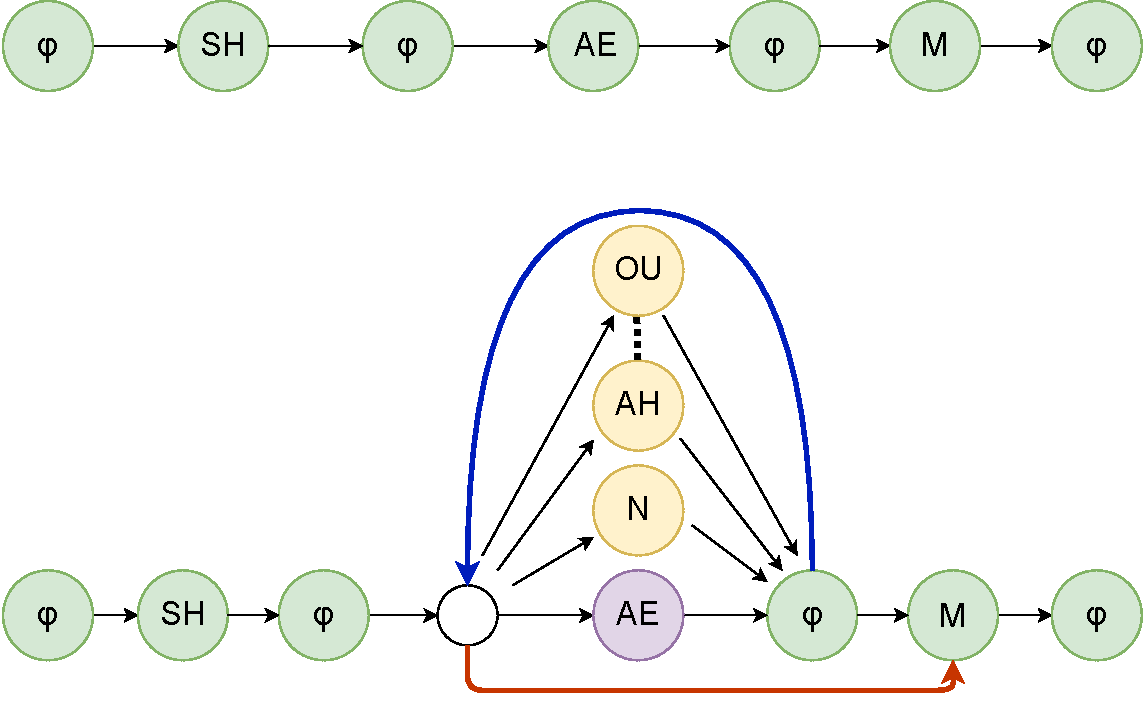
\includegraphics[width=0.97\columnwidth]{figs/final_af_graph.drawio.pdf} 
      \caption{The figure exemplifies the computation of GOP-SF (Eq.~\ref{eq:gop-sf_implementation}) using a CTC-trained model.
      In the example, $\mathcal{L}_{\text{CTC}}(\Lcano, O_1^T)$ can be computed using the graph at the top, whereas $\mathcal{L}_{\text{CTC}}(\Lsdi, O_1^T)$ using the graph at the bottom.
      %The top graph corresponds to the canonical sequence ``SH AE M'' and it can be used to compute the CTC loss for the canonical pronunciation . 
      %The graph below corresponds to the denominator that expands the canonical at the target phoneme ``AE''~(the purple node) with all kinds of mis-pronunciations.
      For the sake of simplicity we omit the skip connections and self-loop connections.}
  \label{fig:af-gragh}
\end{figure}
Instead of committing to a specific segmentation as in standard GOP, in the proposed segmentation-free GOP (GOP-SF) we compute the log posterior for the target phone $l_i$ given the full observation sequence $O_1^T$ and all the phonemes in the left and right context:
\begin{equation}
    \text{GOP-SF}(l_i) = \log\left(p(l_i|O_1^T, \Lleft, \Lright)\right).
    \label{eq:gop-sf_definition}
\end{equation}
This is the same definition that we introduced in \cite{cao24b_interspeech}, although not explicitly written as in Eq.~\ref{eq:gop-sf_definition}, there.

In this work, we also introduce a version of this definition that is normalized by the estimated length of the model activations for the target speech segment:
\begin{equation}
    \text{GOP-SF-Norm}(l_i) = \frac{\log\left(p(l_i|O_1^T, \Lleft, \Lright)\right)}{\mathbb{E}[t_2-t_1|O_1^T, \Lleft, \Lright]}.
    \label{eq:gop-sf_implementation_normalized}
\end{equation}
The reason for this new definition is to reduce the variance of the GOP estimates with the different lengths of the activations.
This is similar to the standard GOP definition of Eq.~\ref{eqa:gop}, where the posterior is normalized by $|t_2-t_1|$ with the following differences: 1) our normalization factor is not related to the length of the target segment, but, rather, to the length of the activations of the model corresponding to the target segment. This accommodates both peaky and non-peaky models; 2) we do not commit to a specific speech segmentation and incorporate the uncertainty in the alignment into our estimation.

In the following subsections, we give theoretical and practical accounts of how to estimate the numerator and denominator in Eqs.~\ref{eq:gop-sf_definition} and \ref{eq:gop-sf_implementation_normalized}.
% In the equation, \Eocc is the expected occupation count for the segment $l_i$ the estimation of which will be detailed in Section~\ref{sec:estimating_duration}.
%It is worth noting that by this definition, the context awareness is increased comparing to the original GOP in Eq.~\ref{eqa:gop}.
\subsection{Segmentation-free target phoneme posterior estimation}
\label{sec:alignment-free_posterior_estimation}
In this section we show how to compute the argument of the log function in Eqs.~\ref{eq:gop-sf_definition} and \ref{eq:gop-sf_implementation_normalized}, that is the alignment-free estimation of the posterior for the target phoneme $p(l_i|O_1^T, \Lleft, \Lright)$.
We first rewrite the expression using the chain rule of probabilities:
\begin{equation}
   p(l_i|O_1^T, \Lleft, \Lright) = \frac{ p(\Lleft, l_i, \Lright|O_1^T)}{p(\Lleft, \Lright|O_1^T)}.
   \label{eq:gop-sf_first_expansion}
\end{equation}

We now consider a specific alignment $(t_1, t_2)$ for the target phone $l_i$ and we define the set of all possible alignments as
\begin{equation}
    \SEG(l_i)=\{(t_1,t_2): i-1 < t_1 \leq t_2 < T-(|\Lcano|-i)\}.
\end{equation}
Because the left context $\Lleft$ and the right context $\Lright$ contain respectively $i-1$ and $|L_C|-i$ symbols, 
the lower bound for $t_1$ and the upper bound for $t_2$ ensure that there is at least one frame for each phone in the left and right context.

We can now expand numerator and denominator in Eq.~\ref{eq:gop-sf_first_expansion} by considering the specific alignment ($t_1, t_2$) and by summing over all possible alignments $\SEG(l_i)$:
% \begin{flalign}
%     & p(\Lleft, l_i, \Lright|O_1^T) = \nonumber \\
%     &= \sum_{(t_1, t_2) \in \SEG(l_i)} p(\Lleft, l_i, \Lright|O_1^T, t_1, t_2) p (t_1, t_2|O_1^T), \label{eq:numerator} \\
%     & p(\Lleft, \Lright|O_1^T) = \nonumber \\
%     &=\sum_{(t_1, t_2) \in \SEG(l_i)} p(\Lleft, \Lright|O_1^T, t_1, t_2) p (t_1, t_2|O_1^T).
%     \label{eq:denominator}
% \end{flalign}

\begin{flalign}
    & \frac{p(\Lleft, l_i, \Lright|O_1^T)}{p(\Lleft, \Lright|O_1^T)} = \nonumber \\
    &= \frac{\sum\limits_{(t_1, t_2) \in \SEG(l_i)} p(\Lleft, l_i, \Lright, t_1, t_2|O_1^T)}
    {\sum\limits_{(t_1, t_2) \in \SEG(l_i)} p(\Lleft, \Lright, t_1, t_2|O_1^T)} = \nonumber \\
    &= \frac{\sum\limits_{(t_1, t_2) \in \SEG(l_i)} p(\Lleft, l_i, \Lright|O_1^T, t_1, t_2) p (t_1, t_2|O_1^T)}
    {\sum\limits_{(t_1, t_2) \in \SEG(l_i)} p(\Lleft, \Lright|O_1^T, t_1, t_2) p (t_1, t_2|O_1^T)}.
    \label{eq:gop-sf_second_expansion} 
\end{flalign}

Special attention must be paid to the term $p(t_1, t_2|O_1^T)$ within both sums at the numerator  and denominator  of Eq.~\ref{eq:gop-sf_second_expansion}.
This is the probability of a certain alignment for the $i$th segment, given the observation sequence, but independent of the actual transcription.
We can interpret this as a prior with respect to the transcription over all possible segmentations.
This distribution could be estimated from the training data.
However, in our definition of GOP-SF, we make the simplifying assumption that this distribution is uniform.
Under this assumption $p(t_1, t_2|O_1^T)$ is a constant and can be taken out of the sums and finally cancels out between the numerator and the denominator of Eq.~\ref{eq:gop-sf_second_expansion} which becomes:
\begin{flalign}
    \frac{p(\Lleft, l_i, \Lright|O_1^T)}{p(\Lleft, \Lright|O_1^T)}
    &= \frac{\sum\limits_{(t_1, t_2) \in \SEG(l_i)} p(\Lleft, l_i, \Lright|O_1^T, t_1, t_2)}
    {\sum\limits_{(t_1, t_2) \in \SEG(l_i)} p(\Lleft, \Lright|O_1^T, t_1, t_2) }.
    \label{eq:gop-sf_third_expansion} 
\end{flalign}


%\begin{flalign}
% & p(t_1, t_2|O_1^T, \Lleft, \Lright) \approx \\
% & \frac{p(\Lleft|O_{1}^{t_1-1})p(\Lright|O_{t_2+1}^T)}
%    {\sum_{(t_1, t_2) \in \SEG} \ p(\Lleft|O_{1}^{t_1-1})p(\Lright|O_{t_2+1}^T)}.
%\label{eq:prob_segmentation_approximate}
%\end{flalign}

Finally, the terms within the sums in Eq.~\ref{eq:gop-sf_third_expansion} can be computed with the CTC's forward variables $\alpha$ and $\beta$ as defined in \cite{CTC}:
\begin{flalign}
    \frac{\sum\limits_{(t_1, t_2) \in \SEG(l_i)} \alpha_{t_1-1}(i-1) \left[\prod_{t=t_1}^{t_2} y_t(l_i)\right] \beta_{t_2+1}(i+1)}
    {\sum\limits_{(t_1, t_2) \in \SEG(l_i)} \alpha_{t_1-1}(i-1) \beta_{t_2+1}(i+1)}.
    \label{eq:gop-sf_forward} 
\end{flalign}

In fact, the numerator in Eq.~\ref{eq:gop-sf_forward} is equivalent to the original definition of the CTC loss for the canonical pronunciation \Lcano and the acoustic features $O_1^T$, except for a $-\log(.)$ term.
Similarly, the denominator can be computed with CTC loss if we define a modified canonical pronunciation $\Lsdi$ as:
\begin{align*}
 \Lsdi &= 
 \{
 \underbrace{l_1, \dots, l_{i-1}}_{\Lleft}, 
 \underbrace{.*,}_{\text{any phoneme sequence}} 
 \underbrace{l_{i+1}, \dots, l_{|\Lcano|}}_{\Lright},
 \}.
\end{align*}
This is the set of all possible transcriptions in which the left and right contexts are equal to the canonical transcription, but we allow any sequence of phonemes in place of the target phoneme $l_i$\footnote{In this and later expressions, we have borrowed notation from regular expressions where ``.'' corresponds to any phoneme, ``*'' is zero or more occurrences, and ``?'' is zero or one occurrence.}.
This corresponds to allowing any number of ``substitution'', ``deletion'' and ``insertion'' errors in pronunciation, justifying the SDI subscript.
This CTC loss can be implemented by defining a graph exemplified in Figure~\ref{fig:af-gragh} (bottom) and running the forward algorithm using this graph.

In summary, combining Eqs~\ref{eq:gop-sf_definition} and \ref{eq:gop-sf_forward}, the GOP-SF can be efficiently computed as the difference between the CTC loss for the pair~(\Lsdi,$O_{1}^{T}$) and the CTC loss for~(\Lcano, $O_{1}^{T}$):
\begin{equation}
    \text{GOP-SF}(l_i) = \mathcal{L}_{CTC}(\Lsdi, O_{1}^{T}) - \mathcal{L}_{CTC}(\Lcano, O_{1}^{T}).
    \label{eq:gop-sf_implementation}
\end{equation}


% Under this assumption, our approximated definition of GOP-SF becomes:
% \begin{flalign}
% & \text{GOP-SF}(l_i) \approx \\
% & \log\left(
% \frac{\displaystyle \sum_{(t_1, t_2) \in \SEG} p(\Lleft|O_{1}^{t_1-1})p(l_i|O_{t_1}^{t_2})p(\Lright|O_{t_2+1}^T)}
% {\displaystyle \sum_{(t_1, t_2) \in \SEG} p(\Lleft|O_{1}^{t_1-1})p(\Lright|O_{t_2+1}^T)}
% \right)
% \label{eq:gop-sf_approximate_definition}
% \end{flalign}


% The left term in the sum in Eq.~\ref{eqa:gop-sf_expansion} can be rewritten as:
% \begin{flalign}
%     & p(l_i|O_1^T, \Lleft, \Lright, t_1, t_2) = \nonumber \\
%     &=\frac{p(L_L, l_i, L_R|O_1^T, t_1, t_2)}{p(L_L, L_R| O_1^T, t_1, t_2)}  = \nonumber \\
%     &= \frac{\alpha_{t_1-1}(i-1) \prod_{t=t_1}^{t_2} y_t(l_i) \beta_{t_2+1}(i+1)}{\alpha_{t_1-1}(i-1) \beta_{t_2+1}(i+1)} = \prod_{t=t_1}^{t_2} y_t(l_i),
% \end{flalign}
% Where $\alpha$ and $\beta$ are the forward and backward variables as defined for CTC \cite{CTC}, 

Note that, because we are considering contributions from all possible segmentations, our method is able to deal with uncertainty in alignment.
Also, the definition of \Lsdi with a graph as in Figure~\ref{fig:af-gragh} gives us flexibility on the kind of pronunciation errors we consider.
If the full graph is used, any substitution (S), deletion (D) and insertion (I) errors are considered.
We refer to this version of the method as GOP-SF-SDI.
If we remove the blue path from the graph, we only consider substitutions and deletions (GOP-SF-SD).
This corresponds to a modified canonical pronunciation
\begin{align*}
 \Lsd &= 
 \{
 \underbrace{l_1, \dots, l_{i-1}}_{\Lleft}, 
 \underbrace{.?,}_{\text{any phoneme or empty}} 
 \underbrace{l_{i+1}, \dots, l_{|\Lcano|}}_{\Lright},
 \}.
\end{align*}

If we also remove the red path, we only consider substitutions as in the traditional GOP (GOP-SF-S) and the modified canonical pronunciation is
\begin{align*}
 L_S &= 
 \{
 \underbrace{l_1, \dots, l_{i-1}}_{\Lleft}, 
 \underbrace{.,}_{\text{any phoneme}} 
 \underbrace{l_{i+1}, \dots, l_{|\Lcano|}}_{\Lright},
 \}.
\end{align*}

In \cite{cao24b_interspeech} we used the unnormalized forward variables $\alpha$s to compute $\mathcal{L}_{CTC}(\Lsdi, O_{1}^{T})$ due of implementation issues.
However, this may lead to numerical underflow errors when multiplying probabilities over longer speech segments.
In this paper, we implement a version of the algorithm that uses the normalized forward variables $\hat{\alpha}_{t}(s)$ defined in \cite{CTC} for both terms in Eq.~\ref{eq:gop-sf_implementation}.
When making comparisons, we refer to this version as GOP-SF-numerical.

In the experiments, we also consider alternative methods to compute the loss, besides standard CTC.

%In the framework of the CTC loss, all the terms in the above expression can be computed efficiently by relying on the forward algorithm and the $\alpha$ and $\beta$ variables:
%\begin{align}
%    p(\Lleft|O_1^{t_1-1}) &= \alpha(i\!-\!1,t_1\!-\!1) \\
%    p(\Lright|O_{t_2+1}^{T}) &= \beta(i\!+\!1,t_2\!+\!1) \\
%    p(l_i|O_{t_1}^{t_2}) &= \prod_{t=t_1}^{t_2} p(l_i|o_t).
%\end{align}
%
% The numerator in Eq.~\ref{eq:gop-sf_approximate_definition} is just the probability $p(\Lcano|O_1^T)$ of the canoncial transcription \Lcano given the complete observation sequence $O_1^T$.
% The denominator in Eq.~\ref{eq:gop-sf_approximate_definition} has a simple interpretation if we define a 

% This definition is exemplified in Figure~\ref{fig:af-gragh} where the graph allows for a deletion (red arrow), substitution (any of the yellow nodes), or any number of insertions (the loop defined by the blue arrow).
% The name ``SDI'' refers to substitutions, deletions and insertions.

% Given a particular segmentation $(t_1, t_2)$ and an observation sequence $O_1^T$, we can compute the probability of $\Lsdi$:
% \begin{align}
%     p(\Lsdi|O_1^T, t_1, t_2) = p(\Lleft|O_1^{t_1-1}) p(*|O_{t_1}^{t_2}) p(\Lright|O_{t_2+1}^{T}),
%     \label{eq_prob_lsdi_given_seg}
% \end{align}
% where we have used the fact that the segmentation makes the three terms (\Lleft, $*$ and \Lright) independent.
% Considering the graph in Figure~\ref{fig:af-gragh}, it should be clear that
% \begin{align}
%     p(*|O_{t_1}^{t_2}) = \prod_{t=t_1}^{t_2} p(*|o_t) = 1,
%     \label{eq:prob_star_give_seg}
% \end{align}
% because for every frame we need to sum the posteriors over all the possible output symbols, i.e. $p(*|o_t) = 1, \forall t$.

% Combining Eq.~\ref{eq_prob_lsdi_given_seg} and \ref{eq:prob_star_give_seg} we can see that the term inside the sum at the denominator of Eq.~\ref{eq:gop-sf_approximate_definition} is equivalent to $p(\Lsdi|O_1^T, t_1, t_2)$.
% As a consequence, GOP-SF is the log of the ratio of the probability of the canonical transcription $L_c$ and the probability of $\Lsdi$ given the observation sequence:
% \begin{equation}
%    \text{GOP-SF}(l_i) 
%         = \log\left(\frac{p(\Lcano|O_1^T) }{p(\Lsdi|O_1^T)}\right) 
%    \label{eqn:gop_alignment_free_compact}
% \end{equation}

% In practice, GOP-SF can be efficiently calculated by computing the probabilities based on graph in Figure~\ref{fig:af-gragh} (top) for the numerator and Figure~\ref{fig:af-gragh} (bottom) in the denominator using dynamic programming.

\subsection{Segmentation-free activation length estimation}
\label{sec:estimating_duration}
We now turn to the denominator of Eq.~\ref{eq:gop-sf_implementation_normalized}, that is on the estimation of the model activation length for the target phoneme $\mathbb{E}[t_2-t_1|O_1^T, \Lleft, \Lright]$.

%There are two points that are different from the normalizer $t_2-t_1$ in Eq.\ref{eqa:gop}: 1) \Eocc does not commit to a specific segmentation, i.e. $t_2-t_1$ is a random variable in the above equation and 2) we are not interested in estimating the actual length of the speech segment, but the length of the activations of the acoustic models for the segment.
%The difference should be clear by looking at the right hand plots in Figure~\ref{fig:illustration-alignment-problems}.

We call $\mathcal{N}_{\text{C}}$ the set of central nodes (yellow and purple) in the graph in Figure~\ref{fig:af-gragh} that correspond to the ``.*'' term in \Lsdi.
Then, the expected value of the duration of the activations corresponding to $l_i$, is the sum over the whole observation sequence of the normalized forward variables $\hat{\alpha}$ corresponding to the nodes in $\mathcal{N}_{\text{C}}$:
%We base our estimation of \Eocc on the pre-normalized forward variables stated in Eq.~\ref{eq:normalized-alpha}:
\begin{equation}
    \mathbb{E}[t_2-t_1|O_1^T, \Lleft, \Lright] = \sum_{t=1}^{T}\sum_{s\in \mathcal{N}_{\text{C}}} \hat{\alpha}_t(s) := \text{Occ}(i).
    \label{eq:estimate_occupation}
\end{equation}    
This expression can be efficiently computed with the forward algorithm that is also used to estimate the posterior of the target phoneme $l_i$ detailed in the previous section.
%The estimation of \Eocc can be computed efficiently using the graph for \Lsdi (or \Lsd, or $L_\text{S}$) in Figure~\ref{fig:af-gragh} and the normalized forward algorithm.
Note that the definitions of \Lsdi and \Lsd allow deletion of the target segment as a possible mispronunciation error.
In this case, $\mathbb{E}[t_2-t_1|O_1^T, \Lleft, \Lright]$ will tend to zero and GOP-SF will tend to diverge.
In the actual implementation, therefore, we define a floor value of 1.

We expect this normalization factor to be most relevant for models that are not peaky in time.
Peaky models tend to have activations that span over a single frame, thus making GOP-SF roughly equivalent to GOP-SF-Norm.
%The is the reason of the maximum operation\footnote{If using the normalized forward algorithm as discussed in Sec.\ref{sec:numerical}, the max(.) should include two \Eocc terms from $L_{det}$ and $L_{sub}$ accordingly.} in Eq.~\ref{eq:gop-sf_implementation_normalized} and $\theta$ is a hyper-parameter around one and heuristically $\theta \in [0.5,1.5]$.
%This is because for deletion errors, all the paths for \Lcano will have at least one frame for segmented the deleted phoneme with a very low probability.
% This is not a problem for the mispronunciation detection task that is based on exceeding a threshold, however, special care must be taken in the implementation to avoid numerical errors.
%It is also worth noting that normalizing by \Eocc is less important for acoustic models that exhibit peaky behavior~(POT).
%In this case, the activations for the target phoneme are mostly concentrated in one frame in time and GOP-AF-Norm will be close to GOP-AF. 

% We know that $\bar{\alpha(i,t)}$ represents the probability of a certain state $i$ at time $t$ for the give observations and the graph. 
% The idea of the estimation is, the larger the \Eocc is, the more likely the paths stay in the states $\mathcal{N}_{\text{C}}$ and in turn the larger difference between $\mathcal{L}_{CTC}(\Lsdi)$ and  $\mathcal{L}_{CTC}$ is in \eqref{eq:gop-sf_implementation}.


% To test the validity of Eq.~\ref{eq:estimate_occupation}, we generated examples where we repeat activations for the segment of $l_i$ to simulate different activation lengths.
% Figure~\ref{fig:act-len-sdi} shows \Eocc as functions of the activation length. 
% We randomly pick up the 11th phoneme in utterance ``fabm2aa1'' from CMU Kids and repeat the corresponding segment of activations for that phoneme with the help of forced alignment. 

%Similar to the previous experiment, we then select the model's activation w.r.t. the three phonemes using alignment.
%In order to change the length of activation, we repeat multiple times the model's activation for those frames that are aligned to the middle phoneme.
%As we can see from Fig.\ref{fig:act-len}, the GOP of correct phoneme is invariant to the length of model's activations. 
%On the contrary, for substitution error~(we replace the canonical phoneme /AO/ to /AE/) the GOP is linearly decreased with the number of repetitions of the activation.
%An intuitive normalization can be done with the help of $\Bar{\alpha}$ in Eq.\eqref{eqa:alpha_bar} which closely estimates the number of activations that we repeats, as shown in the blue line in Fig.\ref{fig:act-len}.
%We call this normalization factor for the $i$th symbol as occurrence~(OCC$(i)$) and it is computed by:
%\begin{equation}
%    \text{OCC}(i) = \sum_{t=1}^{T}(\bar{\alpha}(2i+1,t))  
%\end{equation}
%where $2i+1$  represents the expanded state from the graph of of GOP-AF-\textbf{SD} in Fig.\ref{fig:af-gragh} and $\bar{\alpha}(2i+1,t)$ is the normalized forward variable that presents the probability of all non-blank symbols $v \in |V|$ at time step $t$.
%Then we define the normalized alignment-free GOP of the $i$th phoneme as:
%\begin{equation}
%    \text{GOP-AF-norm}(i) = \frac{\text{GOP-AF}(i)}{\max(1, \text{OCC}(i))} 
%\end{equation}
%Note that the occurrence can be less than 1 due to the deletion error, that's the reason why the $max$ operator in the above equation is used.
%The normalized GOP values are plot in Fig.\ref{fig:act-len} with the dashed lines.
%We can see the decreasing trend of GOP over activation length for erroneous phoneme is back into a flat line after doing the normalization. 
%However, it gives only around $0.2\%$ relative improvement of AUC for CE-trained model and no positive benefits for CTC- or EnCTC-trained models.
%It could be explained by CTC/EnCTC-based models usually has unified length of activation regardless of the length of the acoustic segmentation of the speech.
%Another reason is that normalization is only needed for erroneous phoneme as the plot shows and in case of binary classification tasks, a lower GOP for erroneous phoneme actually helps to improve the accuracy. 
%To conclude, there is no need for doing the normalization for binary classification task, and especially for CTC/EnCTC-based models where the activation length is independent of acoustic evidence. 

% We can see from the plot that the estimated number grows linearly with the number of repetitions for both methods. 
% The CTC's POS limits the segment of the target phoneme to only one frame regardless of the actual duration of the phoneme being spoken such that the curves grow approximately at 45 degree angle.
% The curve for GOP-CTC-AF-SDI is less accurate than GOP-CTC-AF-SD due to the reason that \Lsdi allows for as many as insertions in the target state that accepts any possible incoming symbols. 
% The estimated activation length at repetition$=$1 is 1.76, which should be around 1 as the original unrepeated activation.  
% However, the method could count the repetitions correctly as $\text{\Eocc} \approx 1.76 + (n-1)$ for further repetition$=$n.  
% In case of deletion errors when repetition is zero, both methods have a occupation close to zero.
% It indicates that in addition to being a normalization term, we could also use \Eocc as extra information for MDD.
%Estimating \Eocc could provide additional information for MDD:
%For the models whose activations respect acoustic evidence in time, e.g., traditional DNN trained with CE loss, computing \Eocc could be regarded as a robust way to estimate the duration of a target phoneme without performing forced alignment. 
% The robustness is gained by ignoring the correctness of the realization of the phoneme of interest~(due to the use of \Lsdi or \Lsd) but relying on other phonemes in the canonical sequence which are less likely to be pronounced incorrectly. 
%For the models which show POT, e.g., trained with the CTC loss, the duration of a phoneme could not be inferred, however, the class of mispronunciation could be diagnosed. 
%For CTC trained models, we find that the deletion errors often show very small values of \Eocc~(close to zero) whereas for substitution errors or correct pronunciations $\Eocc \in [1,2]$ and for insertions it is often $\Eocc >2$.



% \begin{figure}[t]
%   \centering \includegraphics[width=1\columnwidth]{figs/occ_sd+sdi.png} 
%       \caption{The estimated activation length of the 11th phoneme /AO/ in ``fabm2aa1'' of CMU Kids.}
%   \label{fig:act-len-sdi}
% \end{figure}

% \begin{figure}[t]
%   \centering \includegraphics[width=1\columnwidth]{figs/occ_sd.png} 
%       \caption{The estimated activation length of the 11th phoneme /AO/ in ``fabm2aa1'' of CMU Kids}
%   \label{fig:act-len-sd}
% \end{figure}

\subsection{Computational complexity}
We can compute the complexity of calculating GOP-SF (Eq.~\ref{eq:gop-sf_implementation}) with the help of dynamic programming.
First we note that we only need to evaluate the CTC loss twice, once for the first term $\mathcal{L}(\Lcano, O_1^T)$ and once for the second term $\mathcal{L}(\Lsdi, O_1^T)$ in Eq.~\ref{eq:gop-sf_implementation}.
The graph used to compute $\mathcal{L}(\Lcano, O_1^T)$ (Figure~\ref{fig:af-gragh}, top) contains $|G| = 2|\Lcano|+1$ nodes (the transcription labels interleaved by $\phi$s).
The graph used to compute $\mathcal{L}(\Lsdi, O_1^T)$ (Figure~\ref{fig:af-gragh}, bottom) contains $|G| = 2|\Lcano| + |V|$ nodes, where $V$ is the set of output symbols from the neural network.
The complexity of running dynamic programming on these graphs is therefore $O(T\times |G|) = O(T\times (|\Lcano|+|V|))$, that is, it is linear both in the length of the utterances, in the number of symbols in the canonical transcription augmented by the number of output symbols, which is usually a constant.
For GOP-SF-Norm, the only overhead is the summation in Eq~\ref{eq:estimate_occupation} because the normalized forward variables $\hat{\alpha}$ are already computed.
%It is worth mentioning that with the help of dynamic programming, the complexity of calculating the denominator is $O(|T|\times (|V|+|\Lcano|)$ instead of $O(|T|\times |\Lcano|)$. 
%The latter is the complexity of computing the original CTC loss.


\subsection{Segmentation-free GOP features}
Similarly to the approaches in~\cite{weigthed-GOP, improved_DNN, WEI2009896}, the GOP-SF of the $i$th phoneme in a canonical sequence can be expanded into a feature vector using LPP~(log posterior probability) and \textbf{LPR}~(log posterior ratio vector):
\begin{equation}
   \label{eqa:af-feature}
   \textbf{FGOP-SF}(l_i) = \{\text{LPP}, \textbf{LPR}(l_i)\} 
\end{equation}
where $\text{LPP} = \log\mathit{p}(\Lcano|O_1^T) = -\mathcal{L}_{\text{CTC}}(\Lcano)$ follows the definition of CTC's log-posterior in Eq.\eqref{eqa:CTC-loss} and \textbf{LPR} is a vector of length $|C|+1$:
\begin{equation}
    \label{eqa:LPP}
    \textbf{LPR}(i) = \left\{\log\left(\frac{\mathit{p}(\Lcano|O_1^T)}{p(L | O_1^T)}\right) \text{ with } L \in \Lsd(l_i) \right\}
\end{equation}
where $\Lsd(l_i)$ has already been defined in Section~\ref{sec:alignment-free_posterior_estimation}.
We do not include insertion errors here because that would result in infinite length for the feature vectors.
Similar to GOP-SF-Norm, we append the expected activation count in Eq.~\ref{eq:estimate_occupation} as an extra dimension of the feature vector which forms:
\begin{equation}
   \label{eqa:af-feature}
   \textbf{FGOP-SF-Norm}(l_i) = \{\text{LPP}, \textbf{LPR}(l_i), \text{Occ}(i)\}. 
\end{equation}

The feature vectors can be fed into multi-dimensional MDD classification models that take the feature vectors as input.
%The feature vector of FGOP-F-CTC-AF extracted by~\cite{cao24b_interspeech}, has achieved $0.618\pm0.003$ in Pearson Correlation Coefficient (PCC) using the GOPT~\cite{GOPT} MDD model for the dataset speechocean762\cite{speechocean762}. 
%As far as we know, it is the best phoneme-only task with the state-of-the-art MDD model of GOPT on this dataset. 
%The feature vectors can also be used as diagnosis of the mispronunciations.
%One could use the index of the vector, where the LPP is relatively high, to tell weather it is a correct realization of the sound, or a deletion error, or substitutions to any  specific phonemes. 

\subsection{Measures of Peakiness}
In Section~\ref{sec:alignment_issues}, we have introduced the peaky behavior of CTC-trained models both with respect to time (POT) and symbols (POS).
%and according to our discussion in Section~\ref{sec:Methods},  the relationship between peakiness and the performance of the GOP can be summarized as follow:
Our two methods were introduced in part to cope with this behavior.
Due to the definitions given in Section~\ref{sec:Methods}, we expect the performance of GOP-SA (self-alignment) to increase with both POT and POS, in contrast to standard methods.
We also expect GOP-SF (segmentation-free) to be less affected by POT and POS.
In order to test the effect of POS and POT on the different GOP methods in a reproducible way, 
%On one hand, for GOP-SA, we believe that both POS and POT are the reasons of robustness towards mispronunciations for GOP-CTC-Align.
%The more POT and POS the model is, the information becomes more separated and the better GOP-CTC-Align performs.
%On the other hand, for GOP-CTC-AF, we believe it is less affected by alignment issues because it accounts on all paths of alignments based on the certainty of each alignment.
%The less POS the model has, the more sparsely the alignment paths distribute, and the more advantages the methods shows.
%
%Given the hypothesis, we perform the experiments to analyze the impact of peakiness for various definitions of GOPs using various models of difference level of peakiness.  
we define objective measures of POS and POT.
%separately, because we believe POS and POT are two factors that might influence the GOP differently.
 
%\subsection{Measure for POT: The Blank Coverage~(BC)}
POT, can be measured by the frequency of activation of the blank symbols~($\phi$).
To estimate this, we use the average of post-softmax activation for $\phi$ over the speech dataset $\mathcal{D}$ for a given model $\mathcal{M}$:
\begin{equation}
    \text{BC}(\mathcal{D},\mathcal{M}) = \frac{1}{N}\sum_{n=1}^N\frac{1}{T_n}\sum_{t \in T_n}p(\phi|O_t^n;\mathcal{M}),
\end{equation}
where the dataset $\mathcal{D}$ contains $N$ utterances, each represented by a sequence of speech features $O^n$ of length $T_n$ and the corresponding transcriptions $L^n$.
We call this the blank coverage (BC).
High BC corresponds to very short activations of the non-blank output symbols and, therefore, to high peakiness in time (POT).

%\subsection{Measurement for POS: The Conditional Entropy~(ConEn)}
For POS, we borrow the idea from~\cite{CTC-ME} and define the average conditional entropy (ConEn) as:
\begin{equation}
    \text{ConEn}(\mathcal{D},\mathcal{M}) = \frac{1}{N}\sum_{n=1}^N H(p(\pi|L^n,O^n)),
\end{equation}
where
\begin{flalign}
 & H(p(\pi|L^n,O^n)) = \nonumber \\
 &= -\sum_{\pi \in {\{u\in V^{|O|}:\mathcal{B}(u) = L}\}} p(\pi|L^n,O^n)\log p(\pi|L^n,O^n).  
\end{flalign}
Low ConEn corresponds to high peakiness in symbols (POS).